\chapter{Implementasi dan Pengujian}
\label{chap:implementasipengujian}

Pada bab ini akan dibahas mengenai hasil implementasi dan pengujian dari Open Source Snake 360. Permainan ini dapat dimainkan pada \textit{link} ini : https://generaldevilx.github.io/Snake360/

\section{Implementasi}
Pada bagian ini akan dijelaskan mengenai lingkungan yang digunakan untuk membangun dan implementasi antarmuka dari Open Source Snake 360.

\subsection{Lingkungan Perangkat Keras}
Berikut adalah lingkungan perangkat keras yang digunakan dalam pembangunan permainan ini: 

\begin{enumerate}
	\item Perangkat : Laptop
	\item \textit{Processor} : Intel Core i5-7200U 2.5GHz
	\item RAM : 4.00 GB
	\item \textit{Video Card} : GeForce 930MX
	\item Monitor : 14"
	\item \textit{Storage} : 1TB
\end{enumerate}

Pada pengujian digunakan 1 buah perangkat \textit{mobile} berbasis android dan 1 buah perangkat \textit{desktop}. Berikut adalah lingkungan perangkat keras yang digunakan dalam pengujian permainan ini:

\textbf{Perangkat 1}\\
\begin{enumerate}
	\item Perangkat : Laptop
	\item \textit{Processor} : Intel Core i5-7200U 2.5GHz
	\item RAM : 4.00 GB
	\item \textit{Video Card} : GeForce 930MX
	\item Monitor : 14"
	\item \textit{Storage} : 1TB
\end{enumerate}

\textbf{Perangkat 2}\\
\begin{enumerate}
	\item Perangkat : SM-J730G
	\item \textit{Processor} : Exynos 7870 Octa 1600MHz Cortex-A53
	\item RAM : 3.00 GB
	\item \textit{Video Card} : Mali-T830
	\item Monitor : 5.5"
	\item \textit{Storage} : 32 GB
\end{enumerate}

\subsection{Lingkungan Perangkat Lunak}
Berikut adalah lingkungan perangkat lunak yang digunakan dalam pembangunan permainan ini:

\begin{enumerate}
	\item Sistem Operasi Laptop : Windows 10 64-bit
	\item Bahasa Pemrograman : \textit{Javascript}, HTML
	\item Sistem Operasi \textit{Smartphone} : Android Nougat v7.0
\end{enumerate}

\subsection{Implementasi Antarmuka}
Pada subbab ini akan ditampilkan dan dijelaskan tampilan antarmuka dari Open Source Snake 360. 

\subsubsection{Tampilan Menu Utama}
Gambar~\ref{fig:GUIUtama} dan Gambar~\ref{fig:GUIUtamaAndroid} merupakan tampilan antarmuka menu utama pada \textit{desktop} dan \textit{smartphone}. Pada tampilan ini terdapat judul dari permainan, \textit{input} untuk mengisi \textit{level} labirin, kecepatan ular berbelok, kecepatan ular, dan tombol '\textit{Play Game}'. Jika pemain salah memasukkan data, maka terdapat pesan kesalahan yang ditandai dengan tulisan bewarna merah. Misal, pada Gambar~\ref{fig:GUIUtamaSalah}, pemain salah memasukkan data untuk level labirin sehingga muncul pesan kesalahan bahwa \textit{input} yang dimasukkan salah.

\begin{figure}[H]
	\centering  
	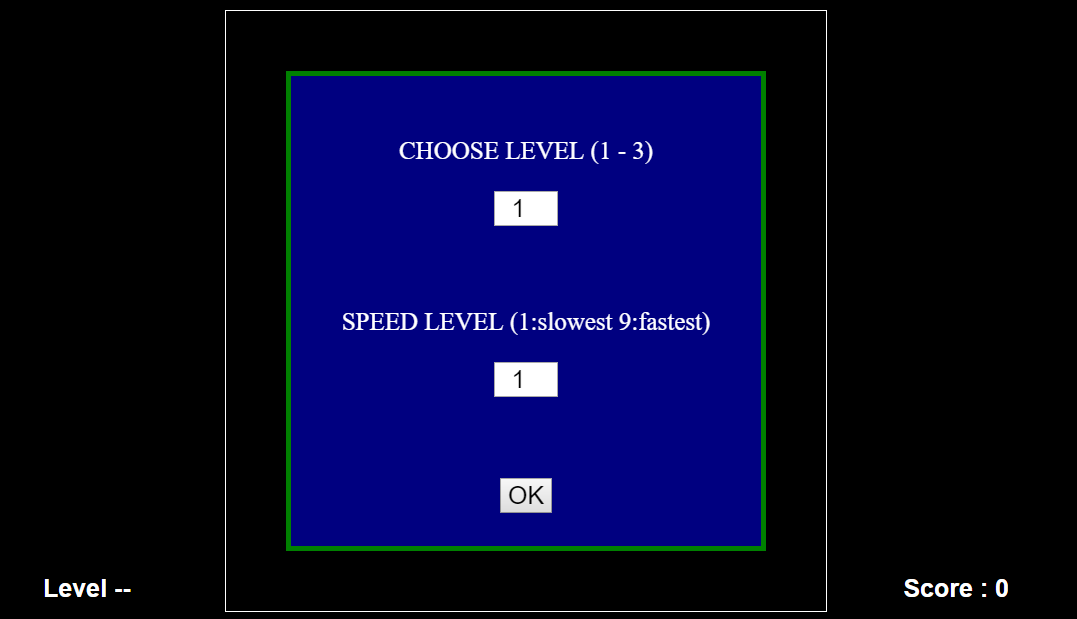
\includegraphics[scale=0.4]{GUIUtama}  
	\caption[Tampilan menu utama pada \textit{desktop}]{Tampilan menu utama pada \textit{desktop}}
	\label{fig:GUIUtama} 
\end{figure}

\begin{figure}[H]
	\centering  
	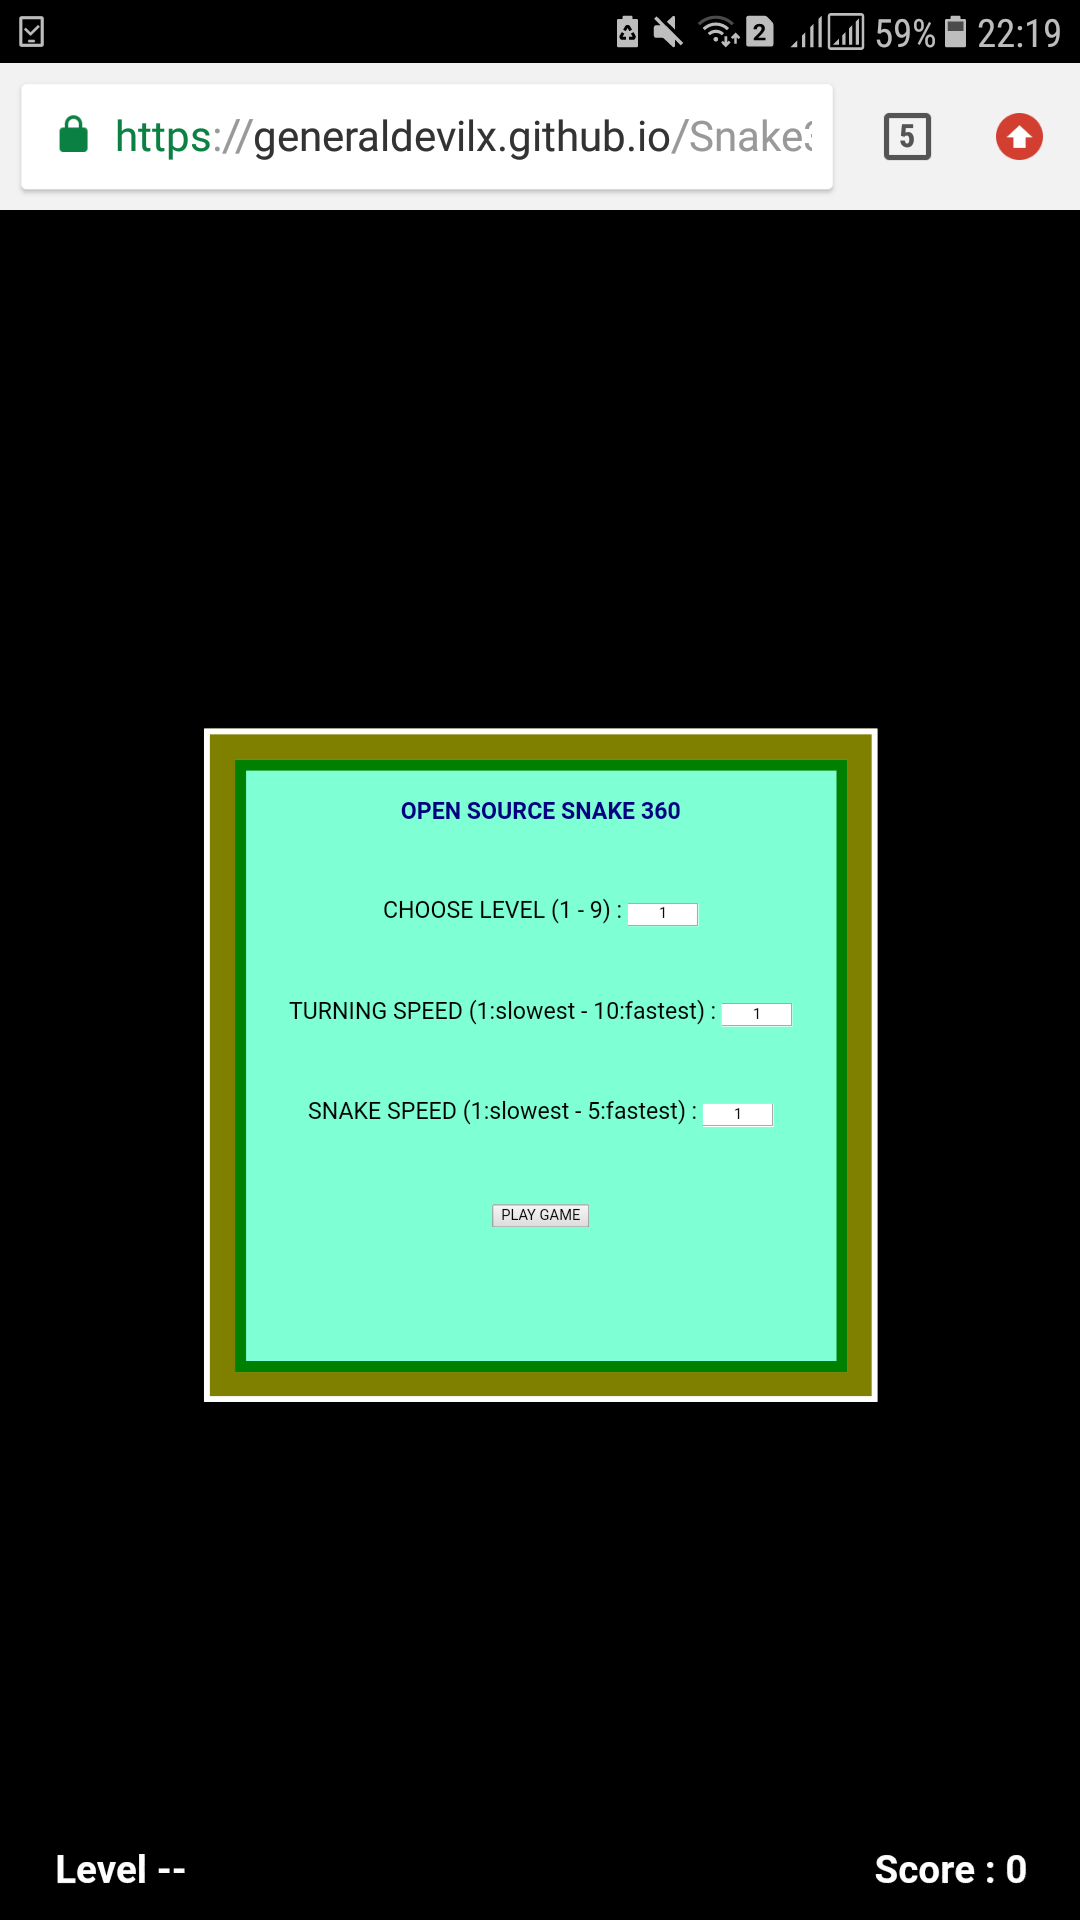
\includegraphics[scale=0.2]{GUIUtamaAndroid}  
	\caption[Tampilan menu utama pada \textit{smartphone}]{Tampilan menu utama pada \textit{smartphone}}
	\label{fig:GUIUtamaAndroid} 
\end{figure}

\begin{figure}[H]
	\centering  
	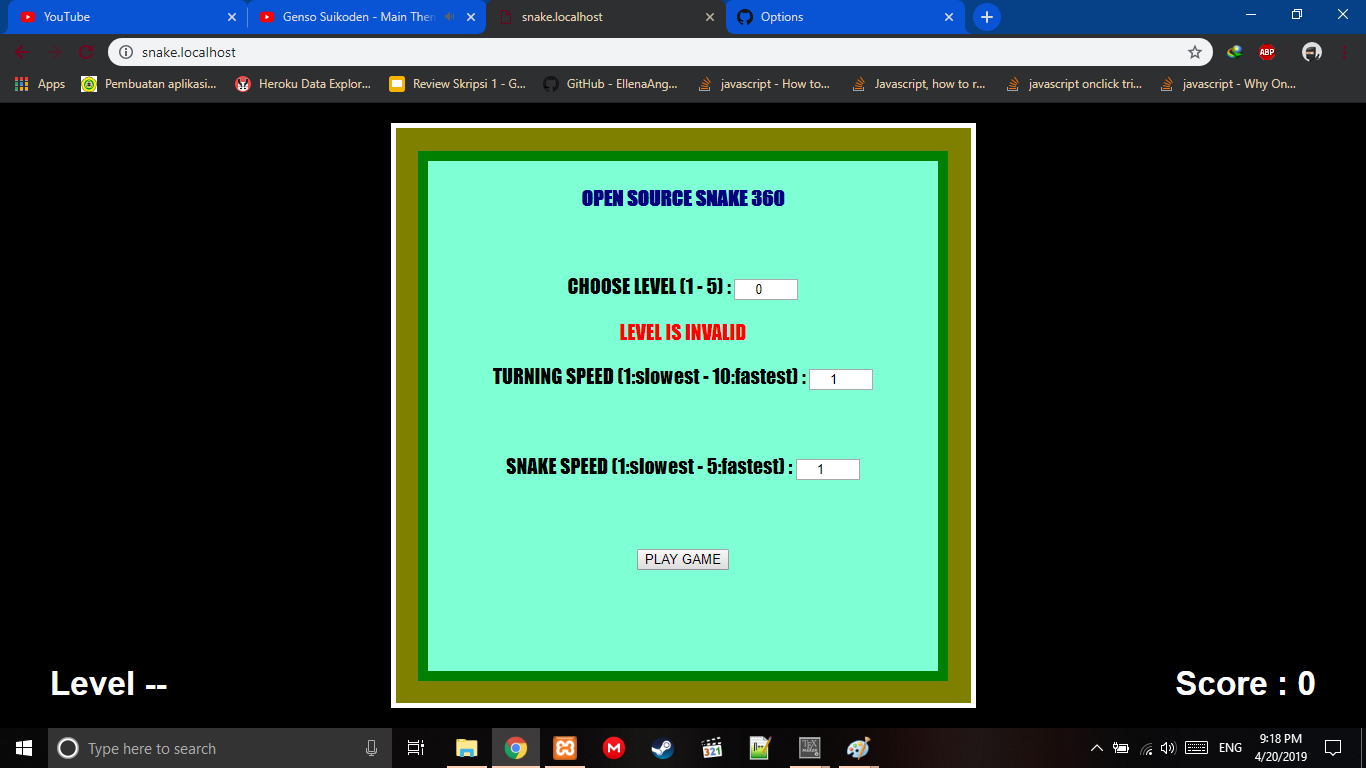
\includegraphics[scale=0.4]{GUIUtamaSalah}  
	\caption[Tampilan menu utama jika pemain salah memasukkan data \textit{level} labirin]{Tampilan menu utama jika pemain salah memasukkan data \textit{level} labirin}
	\label{fig:GUIUtamaSalah} 
\end{figure}

\subsubsection{Tampilan Bermain}
Gambar~\ref{fig:GUIBermain} dan Gambar~\ref{fig:GUIBermainAndroid} merupakan tampilan antarmuka mulai bermain pada \textit{desktop} dan \textit{smartphone}. Tampilan ini muncul apabila pemain memasukkan data level labirin, kecepatan ular berbelok dan kecepatan ular dengan benar dan menekan tombol "\textit{Play Game}". Pada tampilan ini terdapat ular yang dikontrol oleh pemain, dinding labirin, makanan ular, \textit{level} labirin dan skor yang didapat pemain.

\begin{figure}[H]
	\centering  
	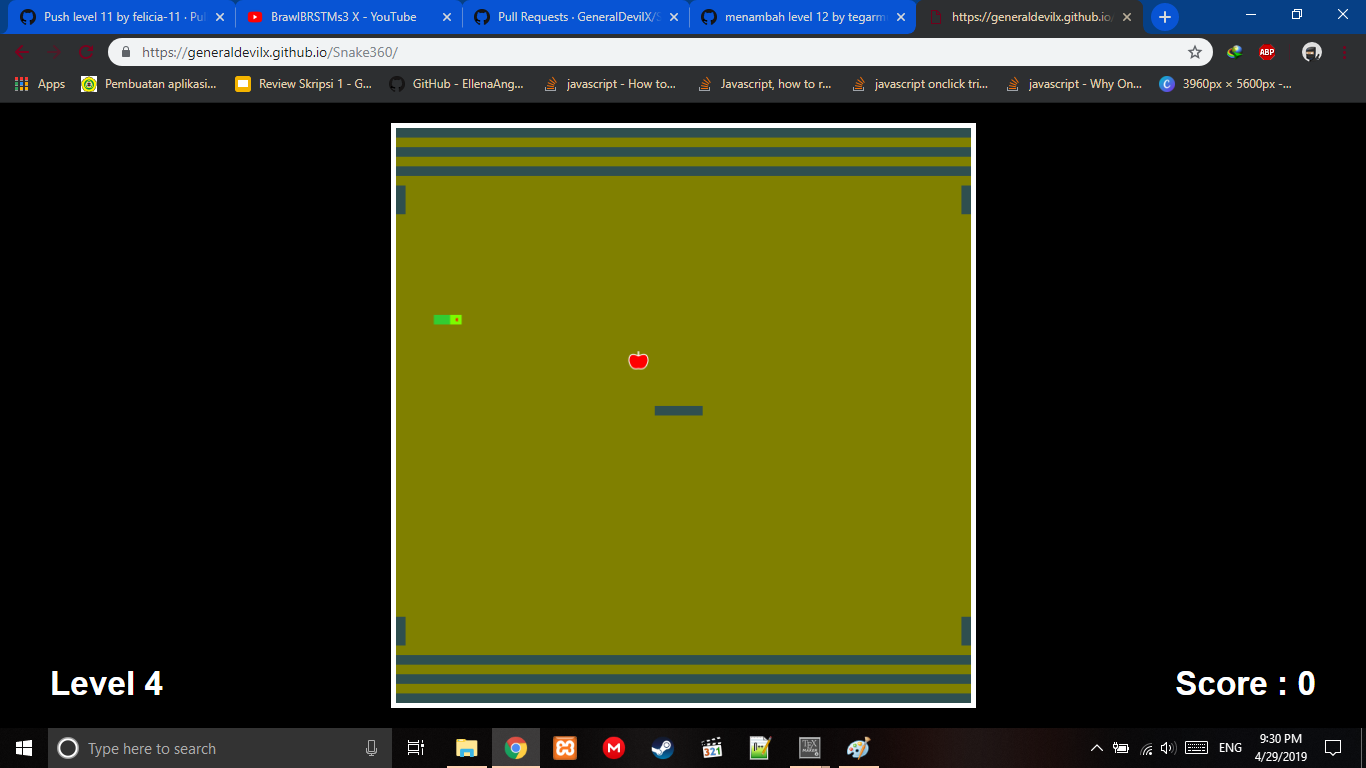
\includegraphics[scale=0.4]{GUIBermain}  
	\caption[Tampilan bermain pada \textit{desktop}]{Tampilan bermain pada \textit{desktop}}
	\label{fig:GUIBermain} 
\end{figure}

\begin{figure}[H]
	\centering  
	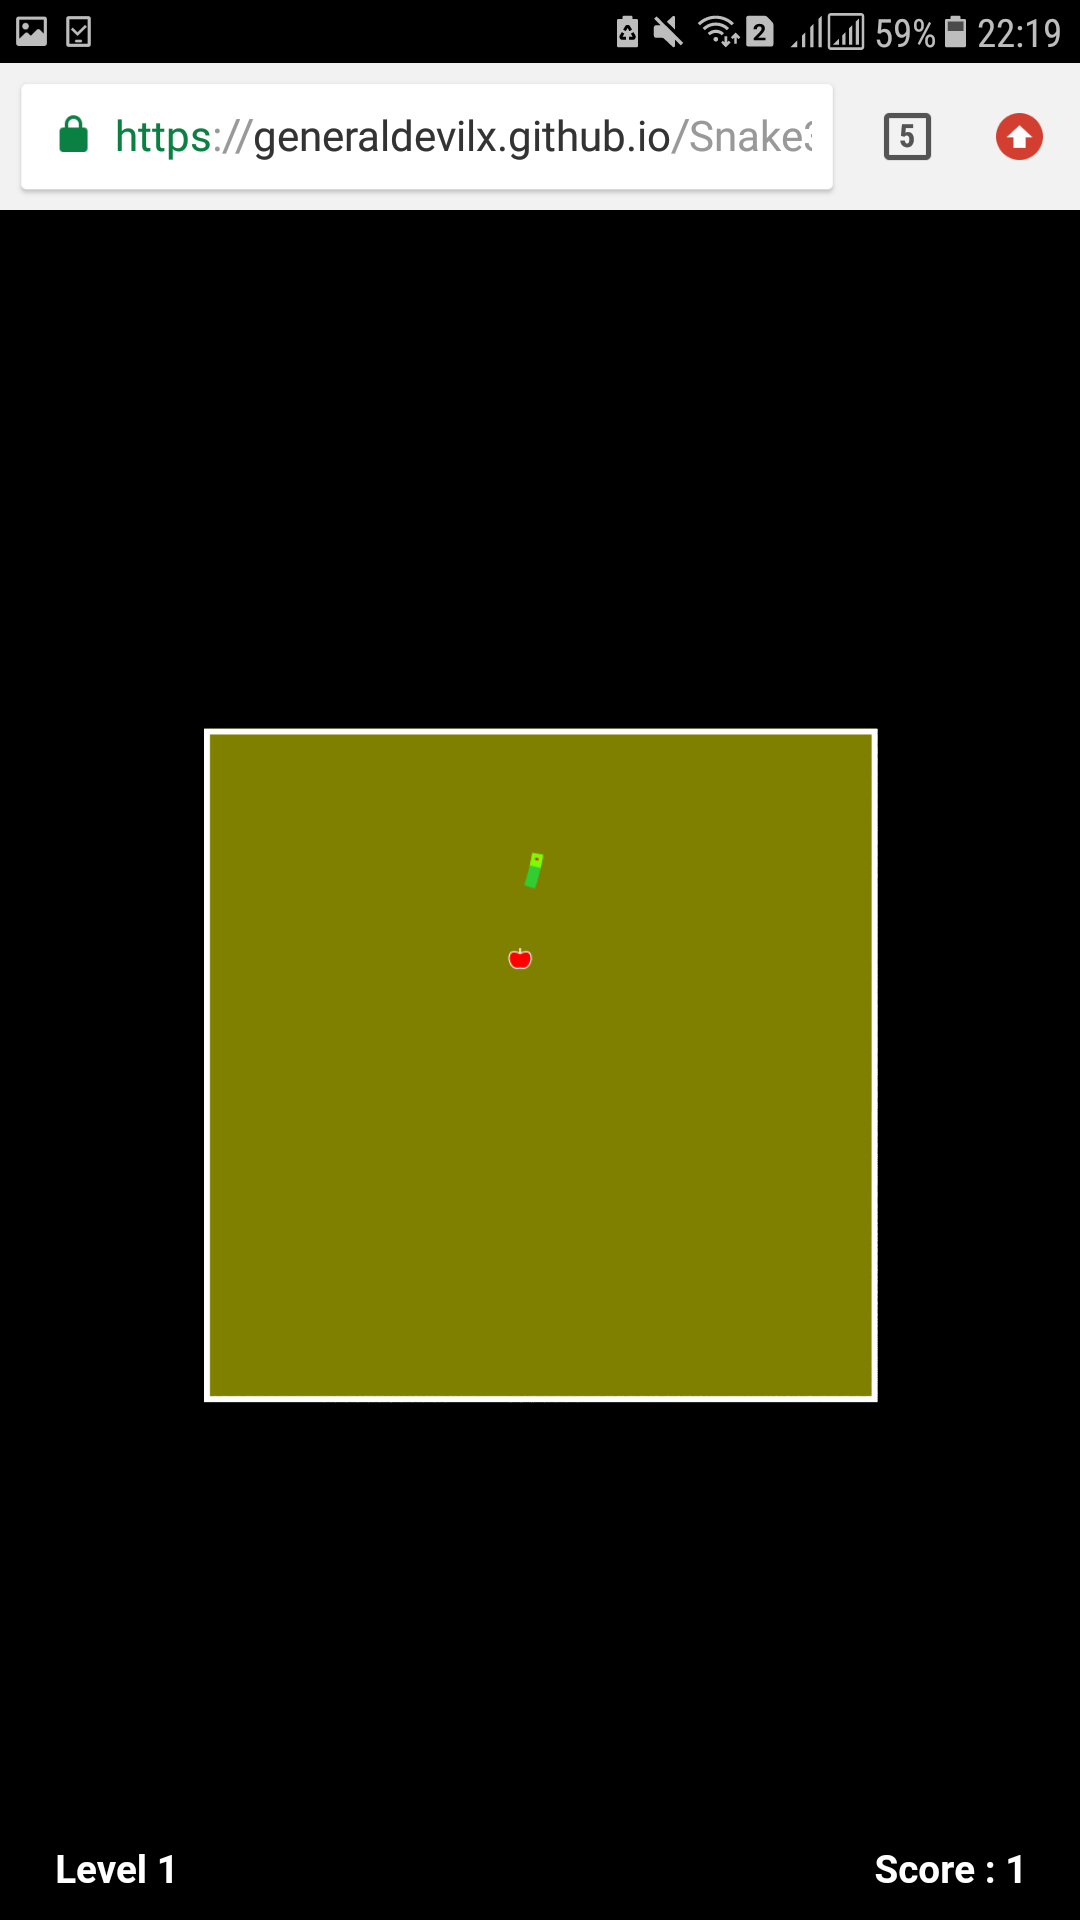
\includegraphics[scale=0.2]{GUIBermainAndroid}  
	\caption[Tampilan bermain pada \textit{smartphone}]{Tampilan bermain pada \textit{smartphone}}
	\label{fig:GUIBermainAndroid} 
\end{figure}

\subsubsection{Tampilan Permainan Berakhir}
Gambar~\ref{fig:GUIBerakhir} dan Gambar~\ref{fig:GUIBerakhirAndroid} merupakan tampilan antarmuka jika permainan berakhir. Tampilan ini muncul apabila ular menabrak dinding labirin dan menabrak tubuhnya sendiri. Pemain akan diarahkan ke tampilan utama jika pemain menekan tombol '\textit{Enter}' pada tampilan ini.

\begin{figure}[H]
	\centering  
	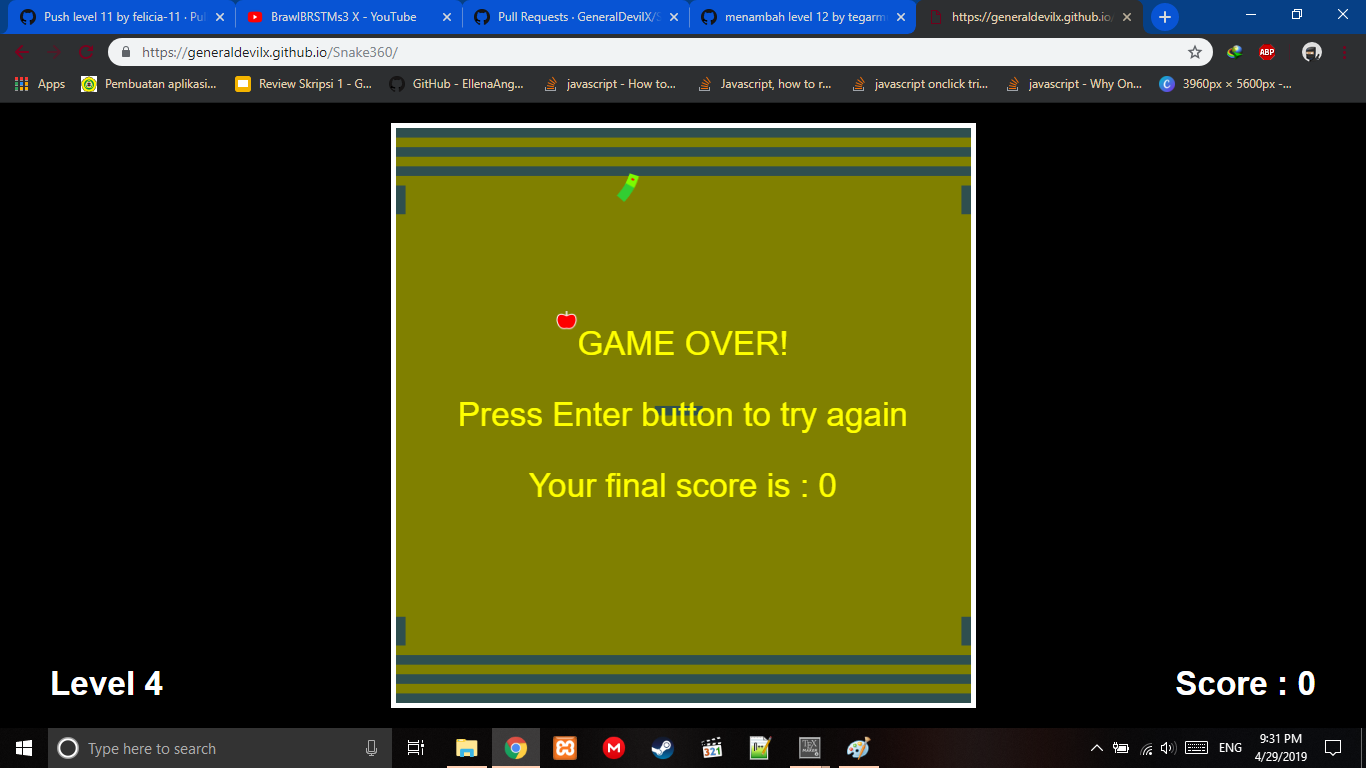
\includegraphics[scale=0.4]{GUIBerakhir}  
	\caption[Tampilan permainan berakhir pada desktop]{Tampilan permainan berakhir pada desktop}
	\label{fig:GUIBerakhir} 
\end{figure}

\begin{figure}[H]
	\centering  
	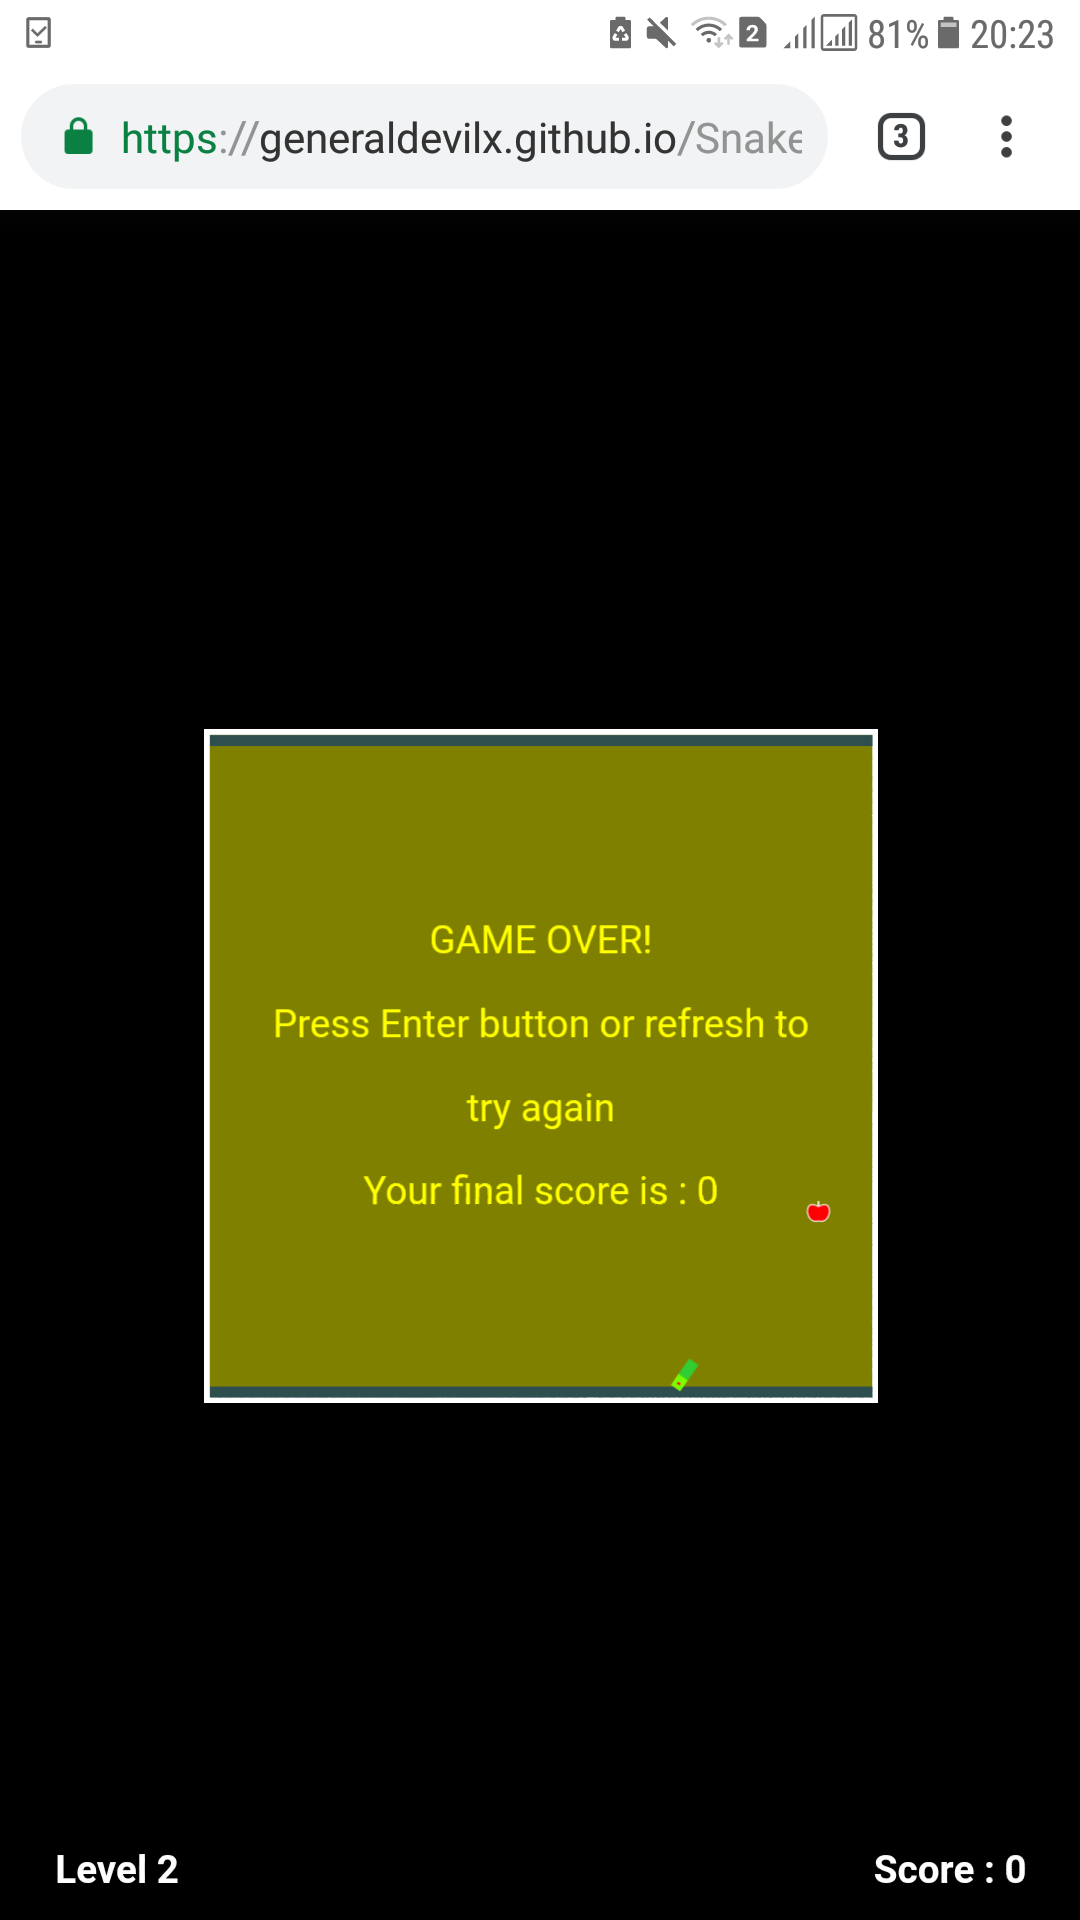
\includegraphics[scale=0.2]{GUIBerakhirAndroid}  
	\caption[Tampilan permainan berakhir pada smartphone]{Tampilan permainan berakhir smartphone}
	\label{fig:GUIBerakhirAndroid} 
\end{figure}

\section{Pengujian}
Pengujian terhadap permainan Open Source Snake 360 ini bertujuan untuk mengetahui apakah permainan yang dibangun sudah berjalan sesuai dengan rancangan. Pengujian yang dilakukan meliputi pengujian fungsional dan pengujian eksperimental. 

\subsection{Pengujian Fungsional}
Pengujian fungsional dilakukan untuk mengetahui tingkat keberhasilan perangkat lunak menjalankan fungsi-fungsi yang ada. Berikut akan ditunjukan pengujian pada tampilan: 

\begin{enumerate}
	\item Pengujian fungsionalitas pada tampilan menu utama.
	
	\begin{table}[H]
		\caption{Pengujian Fungsional pada Tampilan Menu Utama} \label{tab:table1}
		\begin{tabular}{| m{4cm} | m{6cm}  | m{4cm} |}
			\hline
			Kasus uji & Hasil yang diharapkan & Hasil uji \\ \hline
			Pemain memilih labirin dan kecepatan berbelok & Jika pemain salah memasukkan data level labirin, maka akan ditampilkan sebuah text bahwa data yang diisi tidak valid & Hasil pengujian sesuai dengan yang diharapkan\\ \hline
			Pemain menekan tombol "mulai bermain" & Pemain dapat memulai permainan. Kondisi untuk dapat memulai permainan adalah data level labirn dan kecepatan berbelok sudah valid. & Hasil pengujian sesuai dengan yang diharapkan\\ \hline
		\end{tabular}
	\end{table}
	
	Berdasarkan tabel~\ref{tab:table1}, dapat disimpulkan bahwa kasus uji pada tampilan menu utama membawakan hasil sesuai dengan yang diharapkan. 
	
	\item Pengujian fungsionalitas tampilan bermain pada \textit{desktop}.
	
	\begin{table}[H]
		\caption{Pengujian Fungsional Tampilan Bermain pada Desktop} \label{tab:table2}
		\begin{tabular}{| m{4cm} | m{6cm}  | m{4cm} |}
			\hline
			Kasus uji & Hasil yang diharapkan & Hasil uji \\ \hline
			Tombol arah kiri ditekan & Ular akan bergerak melawan arah jarum jam & Hasil pengujian sesuai dengan yang diharapkan\\ \hline
			Tombol arah kanan ditekan & Ular akan bergerak searah jarum jam & Hasil pengujian sesuai dengan yang diharapkan\\ \hline
			Ular memakan apel & Pemain akan mendapatkan skor & Hasil pengujian sesuai dengan yang diharapkan\\ \hline
			Ular menabrak dinding & Tampilan "game over" akan muncul & Hasil pengujian sesuai dengan yang diharapkan\\ \hline
			Ular menabrak tubuh sendiri & Tampilan "game over" akan muncul & Hasil pengujian sesuai dengan yang diharapkan\\ \hline 
		\end{tabular}
	\end{table}
	
	Berdasarkan tabel~\ref{tab:table2}, dapat disimpulkan bahwa kasus uji tampilan bermain pada desktop membawakan hasil sesuai dengan yang diharapkan. 
	
	\item Pengujian fungsionalitas pada tampilan "\textit{Game Over}" 
	
	\begin{table}[H]
		\caption{Pengujian Fungsional pada Tampilan "\textit{Game Over}"} \label{tab:table3}
		\begin{tabular}{| m{4cm} | m{6cm}  | m{4cm} |}
			\hline
			Kasus uji & Hasil yang diharapkan & Hasil uji \\ \hline
			Tombol "\textit{Enter}" ditekan & Pemain akan diarahkan ke tampilan menu utama & Hasil pengujian sesuai dengan yang diharapkan\\ \hline
		\end{tabular}
	\end{table}
	
	Berdasarkan tabel~\ref{tab:table3}, dapat disimpulkan bahwa kasus uji pada tampilan "game over" membawakan hasil sesuai dengan yang diharapkan. 
\end{enumerate}

\subsection{Pengujian Eksperimental}
Pada pengujian eksperimental akan diuji penambahan labirin oleh orang lain. Pada pengujian ini terdapat 5 orang yang akan menambahkan labirin menggunakan \textit{pull request Github}. Berikut adalah hasil pengujian eksperimental : 

\begin{enumerate}
	\item Penguji 1\\
	Penguji 1 menambahkan labirin level 6 dengan menggunakan pull request berhasil dilakukan seperti yang terlihat pada Gambar~\ref{fig:pullReq1}. Dinding labirin yang dibuat sudah sesuai dengan besar canvas. Namun posisi ular yang dimasukkan tidak sesuai. Posisi ular tersebut berada pada daerah dinding labirin. Hasilnya adalah ketika permainan dimulai, permainan akan berakhir. Gambar~\ref{fig:pengujian1} merupakan hasil pengujian menggunakan labirin yang dibuat oleh penguji 1.
	
	\begin{figure}[H]
		\centering  
		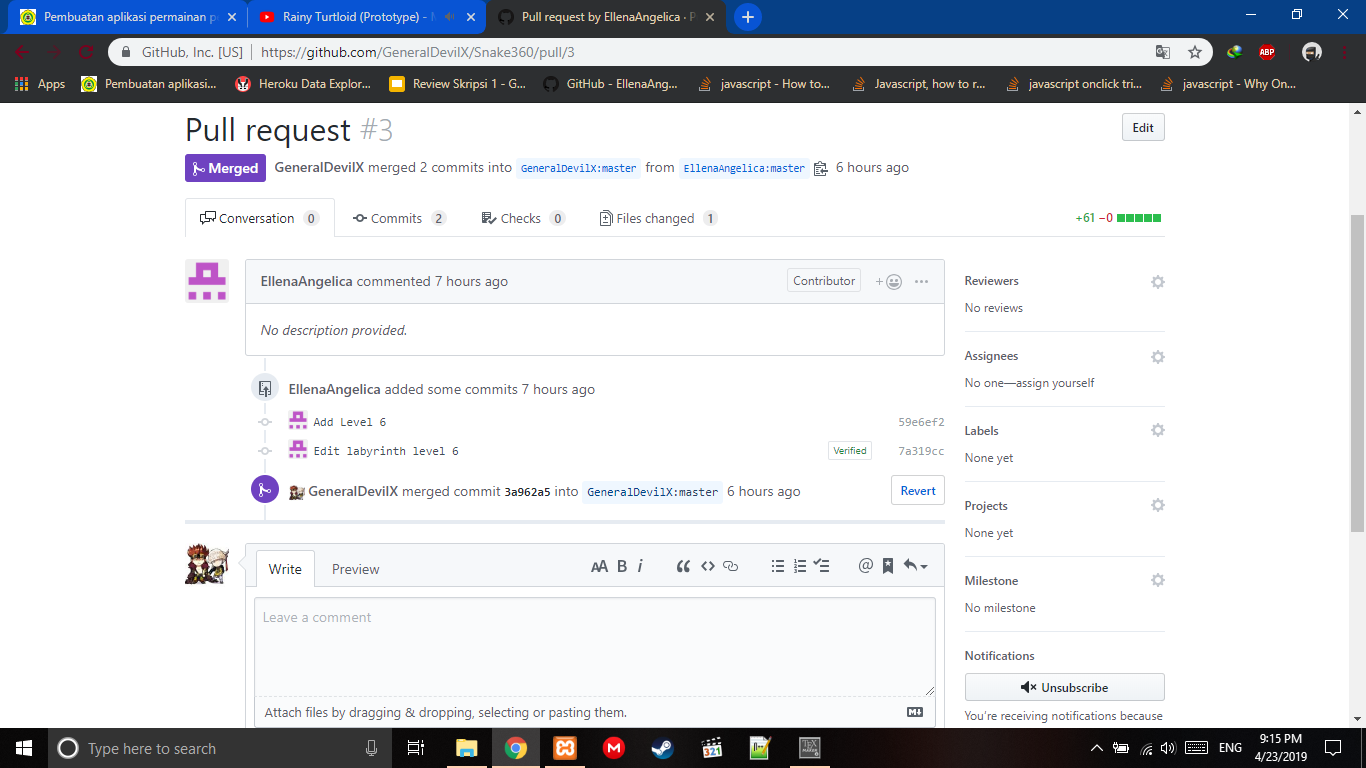
\includegraphics[scale=0.4]{pullReq1}  
		\caption[Tampilan hasil pull request milik penguji 1]{Tampilan hasil pull request milik penguji 1}
		\label{fig:pullReq1} 
	\end{figure}
	
	\begin{figure}[H]
		\centering  
		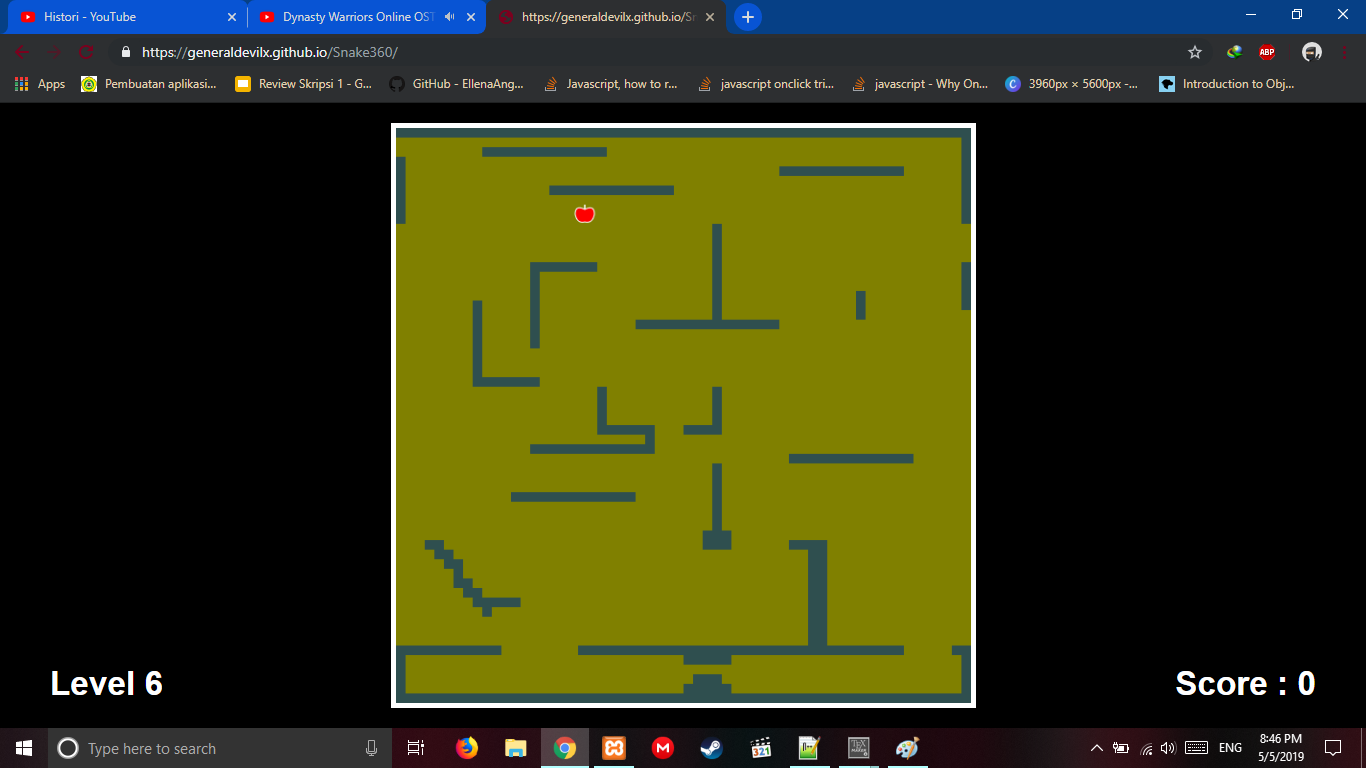
\includegraphics[scale=0.4]{pengujian1}  
		\caption[Tampilan pengujian labirin yang dibuat oleh penguji 1]{Tampilan pengujian labirin yang dibuat oleh penguji 1}
		\label{fig:pengujian1} 
	\end{figure}	
	
	\item Penguji 2\\
	Penguji 2 menambahkan labirin level 7 dengan menggunakan pull request berhasil dilakuka seperti yang terlihat pada Gambar~\ref{fig:pullReq2}. Penguji 2 menambah labirin yang sudah dibuat oleh penguji 1 dan penguji 2 berhasil mengganti nama labirin tersebut. Labirin yang dibuat oleh penguji 2 tidak sesuai dengan besar canvas sehingga tampilan menjadi seperti pada Gambar~\ref{fig:pengujian2}. Penguji 2 membuat labirin yang seluruhnya adalah dinding. Hasilnya sama seperti pengujian 1, pada saat permainan dimulai, permainan akan berakhir.
	
	\begin{figure}[H]
		\centering  
		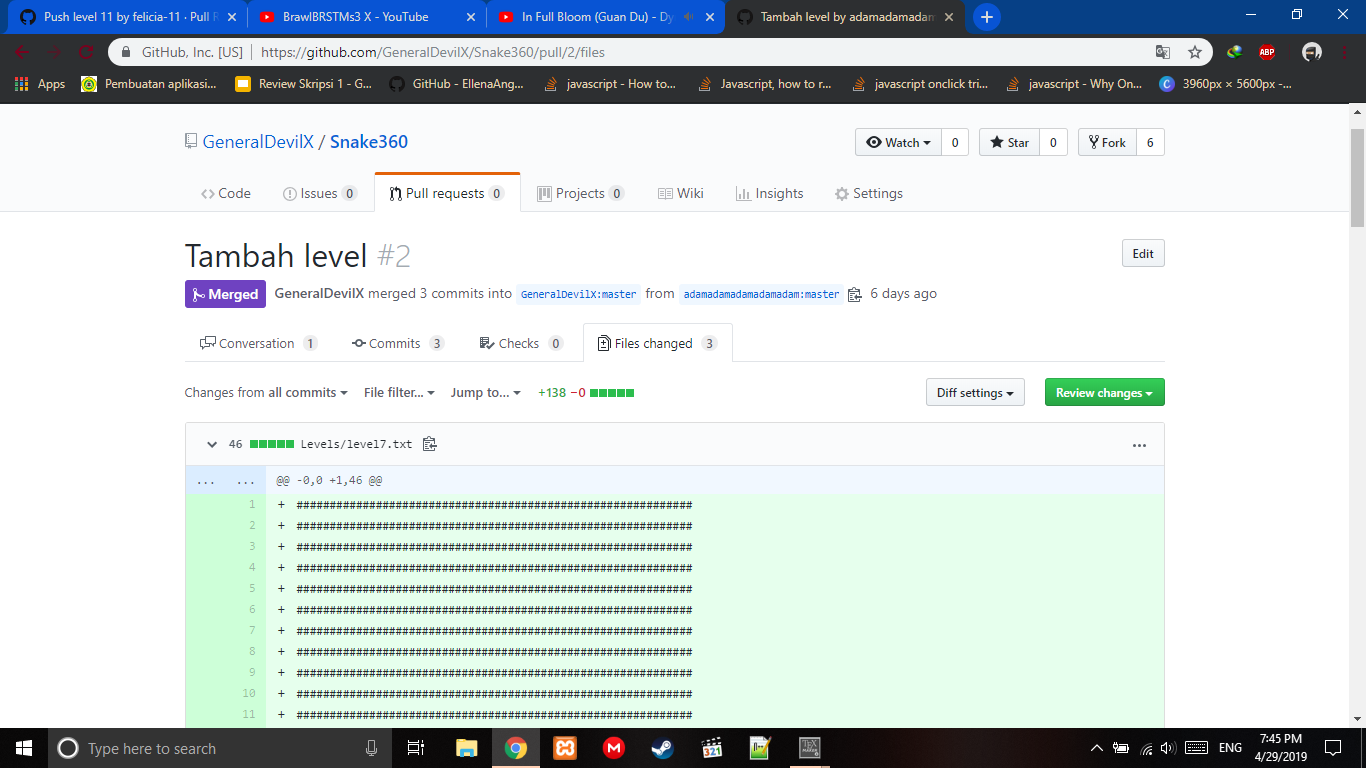
\includegraphics[scale=0.4]{pullReq2}  
		\caption[Tampilan hasil pull request milik penguji 2]{Tampilan hasil pull request milik penguji 2}
		\label{fig:pullReq2} 
	\end{figure}
	
	\begin{figure}[H]
		\centering  
		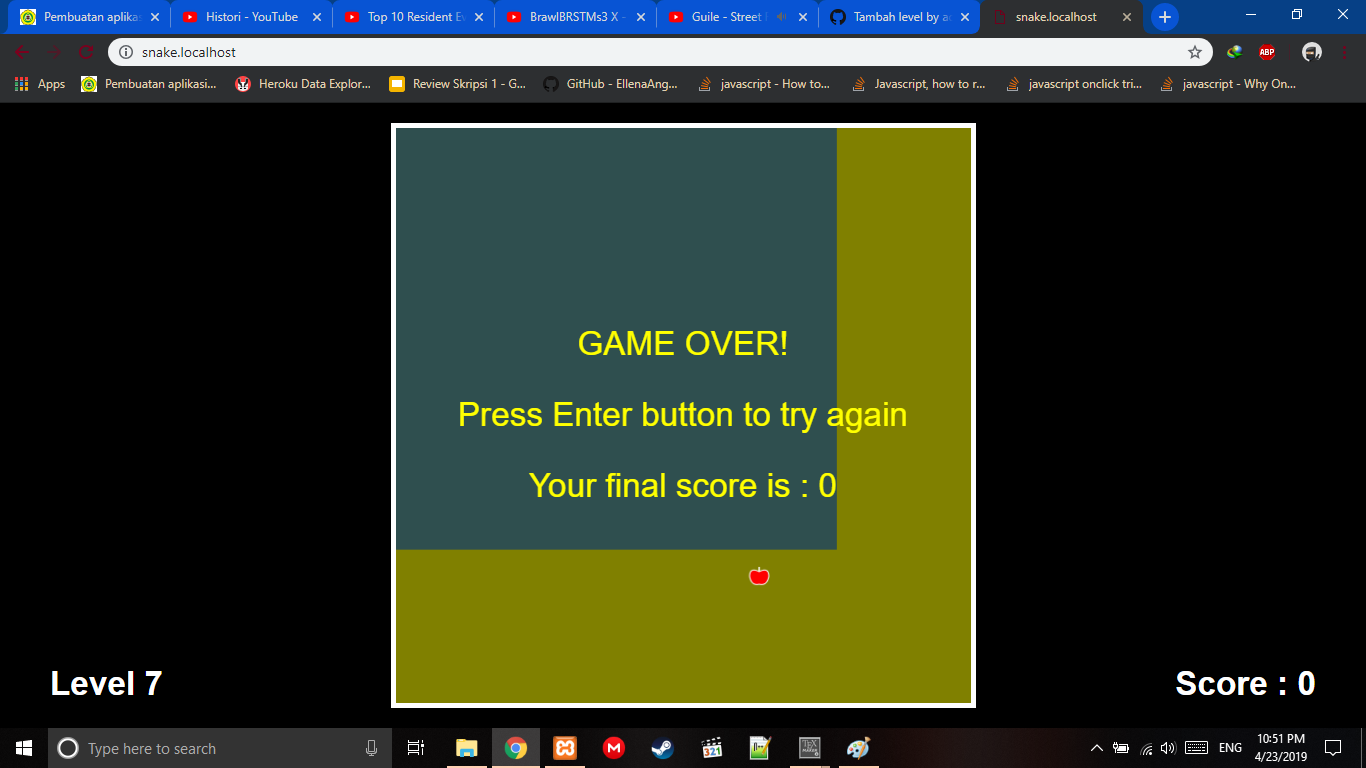
\includegraphics[scale=0.4]{pengujian2}  
		\caption[Tampilan pengujian labirin yang dibuat oleh penguji 2]{Tampilan pengujian labirin yang dibuat oleh penguji 2}
		\label{fig:pengujian2} 
	\end{figure}
	
\end{enumerate}